% Chapter Template

\chapter{Especificació} % Main chapter title

\label{Chapter5} % Change X to a consecutive number; for referencing this chapter elsewhere, use \ref{ChapterX}

Després d'haver explicat l'origen de \textit{Wisebite}, haver estudiat les solucions actuals del mercat i suggerit una de millor i haver analitzat els requisits i les funcionalitats del sistema, cal especificar els models que representaran les entitats que formaran el projecte. En primera instància, es mostrarà l'esquema conceptual que defineix el treball i s'explicarà cada una de les entitats que l'engloben. Per altra banda, s'analitzarà l'esquema de comportament que interacciona entre l'usuari i el sistema.

%----------------------------------------------------------------------------------------
%	SECTION 1
%----------------------------------------------------------------------------------------

\section{Esquema conceptual}

L'esquema conceptual d'un sistema és la representació gràfica dels models que caracteritzen aquest. En Enginyeria del Software això és conegut com un diagrama de classes\cite{diagramaclases}. Primerament, s'explicarà textualment les entitats que participen en l'esquema conceptual i posteriorment es mostrà el diagrama de classes representatiu.

\subsection{Descripció de les classes}

L'esquema conceptual del projecte \textit{Wisebite} disposa de nou classes que s'explicaran a continuació.

\begin{itemize}
\item \textbf{User}: Un usuari és l'entitat que representa a les persones que utilitzaran l'aplicació i les seves funcionalitats. Un usuari té un \textit{id}, que l'identifica, un \textit{correu electrònic} (email), un \textit{nom} (name), un \textit{cognom} (lastName) i una \textit{localització} (location). Cada usuari pot o no tenir una imatge de perfil, treballa o no a un restaurant, pot crear moltes comandes, pot disposar d'un seguit de comandes a valorar i pot tenir d'un conjunt de valoracions realitzades emmagatzemades dins la plataforma.

\item \textbf{Image}: Una imatge és l'entitat que representa una imatge emmagatzemada al sistema. Una imatge té un \textit{id}, que l'identifica, una \textit{ruta} per localitzar-la quan sigui necessari (imageFile) i una \textit{descripció} (description). Cada imatge pot estar relacionada o amb un usuari o bé amb un restaurant.

\item \textbf{Restaurant}: Un restaurant és l'entitat que representa a l'establiment de restauració que engloba l'objectiu de la plataforma. Un restaurant té un \textit{id}, que l'identifica, un \textit{nom} (name), un \textit{telèfon} de contacte (phone), una \textit{descripció} (description), una \textit{localització} (location), un \textit{nombre de taules} (numberOfTables) i la direcció de la \textit{pàgina web} (website). Cada restaurant pot disposar de fins a set horaris d'apertura, pot tenir moltes imatges associades, molts usuaris formant l'equip de treball de l'establiment, pot tenir un conjunt de comandes externes, un conjunt de plats i menús que composen la carta de l'establiment i un grup d'avaluacions realitzades pels usuaris de la plataforma.

\item \textbf{OpenTime}: Un horari d'apertura és l'entitat que representa l'horari d'inici i final d'una franja horària. Un horari d'apertura té un \textit{id}, que l'identifica, un \textit{horari d'inici} (startDate) i un \textit{horari fi} (endDate). Cada horari d'apertura està relacionat amb un restaurant.

\item \textbf{Dish}: Un plat és l'entitat que representa al plat de forma individual. Un plat té un \textit{id}, que l'identifica, un \textit{nom} (name), una \textit{descripció} (description) i un \textit{preu} (price). Cada plat forma part d'un restaurant, pot ser part d'un menú especific jugant el paper de plat principal, secundari o alternatiu, pot tenir un conjunt de valoracions dels usuaris de l'aplicació i forma part d'un seguit de línies de comanda.

\item \textbf{Menu}: Un menu és l'entitat que representa a un menú de la carta de l'establiment. Un menú té un \textit{id}, que l'identifica,un \textit{nom} (name), una \textit{descripció} (description) i un \textit{preu} (price). Cada menú forma part d'un restaurant i pot tenir un conjunt de valoracions dels usuaris de l'aplicació.

\item \textbf{Order}: Una comanda és l'entitat que representa la petició d'un client dins d'un establiment de restauració. Una comanda té un \textit{id}, que l'identifica, una \textit{data} d'inici (date), un \textit{número de taula} (tableNumber) i una \textit{data d'última modificació} (lastDate). Cada comanda es creada per un dels usuaris de la plataforma, pot estar en la llista de comandes a valorar per part d'un usuari, pot ser part del conjunt de comandes externes de l'aplicació i conté un conjunt de línies de comanda.

\item \textbf{OrderItem}: Una línia de comanda és l'entitat que representa un dels elements del llistat que forma una comanda. Una línia de comanda té un \textit{id}, que l'identifica, pot estar o no \textit{preparat} (ready), pot estar o no \textit{estregat} (delivered), pot estar o no \textit{pagat} (paid) i té una \textit{característica diferent} (differentFeature). Cada línia de comanda forma part d'una comanda i té un plat dins del restaurant associat.

\item \textbf{Review}: Una valoració és l'entitat que representa l'opinió d'un usuari sobre un plat, un menú o un restaurant. Una valoració té un \textit{id}, que l'identifica, una \textit{puntuació} (points), un \textit{comentari} (comment) i una \textit{data} de realització (date). Cada valoració està sempre relacionada o bé amb un plat, o amb un menú o amb un restaurant i ha estat realitzada per un usuari.
\end{itemize}

\clearpage
\subsection{Diagrama de classes}

\begin{figure}[!h]
\centering
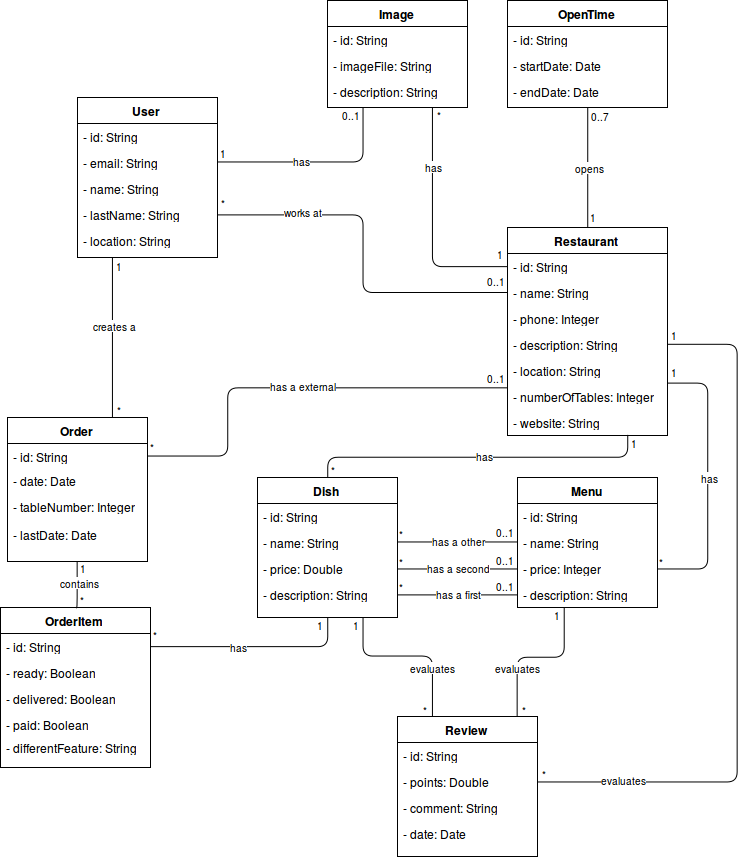
\includegraphics[scale=0.5]{Figures/diagrama_clases.png}
\caption{Diagrama de classes}
\end{figure}

%----------------------------------------------------------------------------------------
%	SECTION 2
%----------------------------------------------------------------------------------------

\clearpage
\section{Esquema del comportament}

Un cop analitzades les classes del model, s'ha de proposar tots els esdeveniments que interaccionen entre l'usuari i el sistema, en els quals es mostrarà inicialment el diagrama de seqüència i el contracte corresponent.
\\

\noindent\textbf{\large Cas d'ús \#1}\\
\begin{figure}[H]
\centering
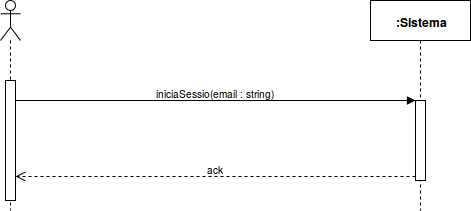
\includegraphics[scale=0.6]{Figures/casdus_01.png}
\caption{Esquema de comportament del cas d'ús \#1}
\end{figure}
\begin{table}[h]
\noindent
\begin{tabularx}{\linewidth}{
>{\hsize=.2\hsize}X% 10% of 4\hsize 
>{\hsize=0.8\hsize}X% 30% of 4\hsize
}
\textbf{Context} 		& Sistema :: iniciaSessio(email : string) \\
\textbf{Precondició} 	& La connexió amb el sistema d'autentificació de Google ha funcionat correctament i el correu electrònic \textit{email} és vàlid.\\
\textbf{Postcondició}	& L'usuari inicia sessió en cas que ja estigues registrat a la plataforma i es crea en cas que no existís. \\
\end{tabularx}
\label{}
\end{table}

\noindent\textbf{\large Cas d'ús \#2}\\
\begin{figure}[H]
\centering
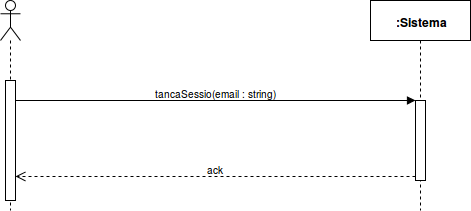
\includegraphics[scale=0.6]{Figures/casdus_02.png}
\caption{Esquema de comportament del cas d'ús \#2}
\end{figure}
\begin{table}[h]
\noindent
\begin{tabularx}{\linewidth}{
>{\hsize=.2\hsize}X% 10% of 4\hsize 
>{\hsize=0.8\hsize}X% 30% of 4\hsize
}
\textbf{Context} 		& Sistema :: tancaSessio(email : string) \\
\textbf{Precondició} 	& La connexió amb el sistema d'autentificació de Google ha funcionat correctament i el correu electrònic \textit{email} existeix a la base de dades. \\
\textbf{Postcondició}	& L'usuari tanca sessió satisfactòriament i deixa de tenir accés a les funcionalitats de la plataforma. \\
\end{tabularx}
\label{}
\end{table}

\clearpage
\noindent\textbf{\large Cas d'ús \#3}\\
\begin{figure}[H]
\centering
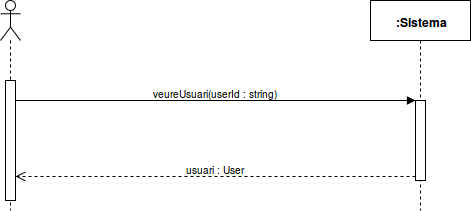
\includegraphics[scale=0.6]{Figures/casdus_03.png}
\caption{Esquema de comportament del cas d'ús \#3}
\end{figure}
\begin{table}[h]
\noindent
\begin{tabularx}{\linewidth}{
>{\hsize=.2\hsize}X% 10% of 4\hsize 
>{\hsize=0.8\hsize}X% 30% of 4\hsize
}
\textbf{Context} 		& Sistema :: veureUsuari(userId : string) \\
\textbf{Precondició} 	& L'usuari amb id \textit{userId} existeix dins la base de dades. \\
\textbf{Postcondició}	& L'aplicació mostra tota la informació relacionada amb l'usuari amb id \textit{userId}. \\
\end{tabularx}
\label{}
\end{table}

\noindent\textbf{\large Cas d'ús \#4}\\
\begin{figure}[H]
\centering
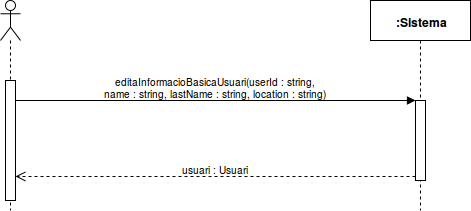
\includegraphics[scale=0.6]{Figures/casdus_04.png}
\caption{Esquema de comportament del cas d'ús \#4}
\end{figure}
\begin{table}[h]
\noindent
\begin{tabularx}{\linewidth}{
>{\hsize=.2\hsize}X% 10% of 4\hsize 
>{\hsize=0.8\hsize}X% 30% of 4\hsize
}
\textbf{Context} 		& Sistema :: editaInformacioBasicaUsuari(userId : string, \\
						& name : string, lastName : string, location : string) \\
\textbf{Precondició} 	& L'usuari amb id \textit{userId} existeix dins la base de dades. \\
\textbf{Postcondició}	& L'aplicació enregistra els canvis i mostra l'usuari modificat. \\
\end{tabularx}
\label{}
\end{table}

\clearpage
\noindent\textbf{\large Cas d'ús \#5}\\
\begin{figure}[H]
\centering
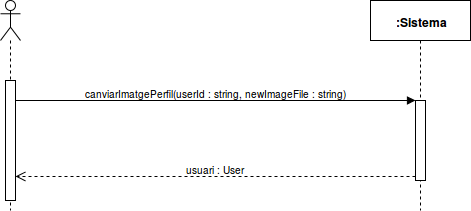
\includegraphics[scale=0.6]{Figures/casdus_05.png}
\caption{Esquema de comportament del cas d'ús \#5}
\end{figure}
\begin{table}[h]
\noindent
\begin{tabularx}{\linewidth}{
>{\hsize=.2\hsize}X% 10% of 4\hsize 
>{\hsize=0.8\hsize}X% 30% of 4\hsize
}
\textbf{Context} 		& Sistema :: canviarImatgePerfil(userId : string, \\
						& newImageFile : string) \\
\textbf{Precondició} 	& L'usuari amb id \textit{userId} existeix dins la base de dades. \\
\textbf{Postcondició}	& L'aplicació emmagatzema la imatge, l'associa a l'usuari i el mostra modificat. \\
\end{tabularx}
\label{}
\end{table}

\noindent\textbf{\large Cas d'ús \#6}\\
\begin{figure}[H]
\centering
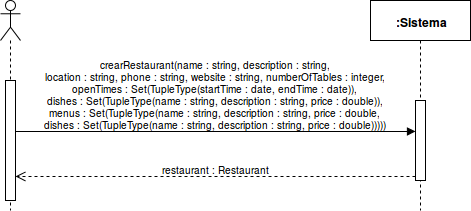
\includegraphics[scale=0.6]{Figures/casdus_06.png}
\caption{Esquema de comportament del cas d'ús \#6}
\end{figure}
\begin{table}[h]
\noindent
\begin{tabularx}{\linewidth}{
>{\hsize=.2\hsize}X% 10% of 4\hsize 
>{\hsize=0.8\hsize}X% 30% of 4\hsize
}
\textbf{Context} 		& Sistema :: crearRestaurant(name : string, description : string, \\
						& location : string, phone : string, website : string, \\
						& numberOfTables : integer, \\
						& openTimes : Set(TupleType(startTime : date, endTime : date)),\\
						& dishes : Set(TupleType(name : string, description : string, \\
						& price : double)), \\
						& menus : Set(TupleType(name : string, description : string, \\
						& price : double, dishes : Set(TupleType(name : string, \\
						& description : string, price : double))))) \\
\textbf{Precondició} 	& - \\
\textbf{Postcondició}	& L'aplicació emmagatzema el restaurant amb els paràmetres indicats i l'associa a l'usuari creador. \\
\end{tabularx}
\label{}
\end{table}

\clearpage
\noindent\textbf{\large Cas d'ús \#7}\\
\begin{figure}[H]
\centering
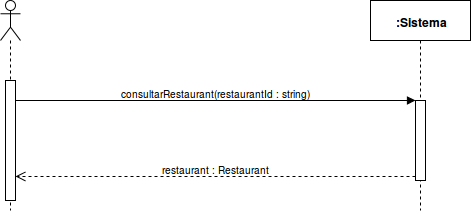
\includegraphics[scale=0.6]{Figures/casdus_07.png}
\caption{Esquema de comportament del cas d'ús \#7}
\end{figure}
\begin{table}[h]
\noindent
\begin{tabularx}{\linewidth}{
>{\hsize=.2\hsize}X% 10% of 4\hsize 
>{\hsize=0.8\hsize}X% 30% of 4\hsize
}
\textbf{Context} 		& Sistema :: consultarRestaurant(restaurantId : string) \\
\textbf{Precondició} 	& El restaurant amb id \textit{restaurantId} existeix dins la base de dades. \\
\textbf{Postcondició}	& L'aplicació mostra tota la informació relacionada amb el restaurant amb id \textit{restaurantId}. \\
\end{tabularx}
\label{}
\end{table}

\noindent\textbf{\large Cas d'ús \#8}\\
\begin{figure}[H]
\centering
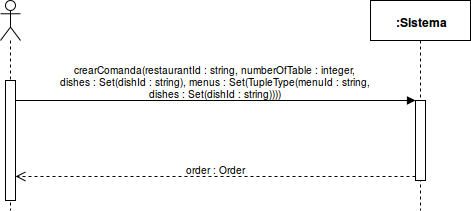
\includegraphics[scale=0.6]{Figures/casdus_08.png}
\caption{Esquema de comportament del cas d'ús \#8}
\end{figure}
\begin{table}[h]
\noindent
\begin{tabularx}{\linewidth}{
>{\hsize=.2\hsize}X% 10% of 4\hsize 
>{\hsize=0.8\hsize}X% 30% of 4\hsize
}
\textbf{Context} 		& Sistema :: crearComanda(restaurantId : string, \\
						& numberOfTable : integer, \\
						& dishes : Set(dishId : string), \\
						& menus : Set(TupleType(menuId : string, \\
						& dishes : Set(dishId : string)))) \\
\textbf{Precondició} 	& El restaurant amb id \textit{restaurantId}, els plats amb id \textit{dishId} i els menus amb id \textit{menuId} existeixen dins la base de dades. \\
\textbf{Postcondició}	& L'aplicació emmagatzema la informació indicada als paràmetres i mostra la comanda creada. \\
\end{tabularx}
\label{}
\end{table}

\clearpage
\noindent\textbf{\large Cas d'ús \#9}\\
\begin{figure}[H]
\centering
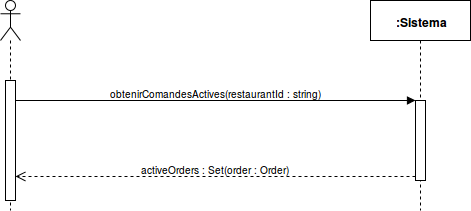
\includegraphics[scale=0.6]{Figures/casdus_09.png}
\caption{Esquema de comportament del cas d'ús \#9}
\end{figure}
\begin{table}[h]
\noindent
\begin{tabularx}{\linewidth}{
>{\hsize=.2\hsize}X% 10% of 4\hsize 
>{\hsize=0.8\hsize}X% 30% of 4\hsize
}
\textbf{Context} 		& Sistema :: obtenirComandesActives(restaurantId : string) \\
\textbf{Precondició} 	& El restaurant amb id \textit{restaurantId} existeix dins la base de dades. \\
\textbf{Postcondició}	& L'aplicació mostra un llistat amb les comandes actives, és a dir, les que encara no han estat finalitzades. \\
\end{tabularx}
\label{}
\end{table}

\noindent\textbf{\large Cas d'ús \#10}\\
\begin{figure}[H]
\centering
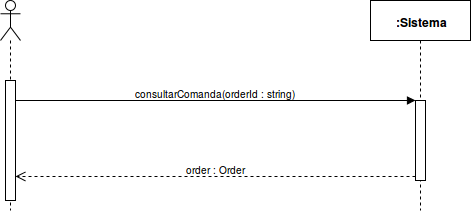
\includegraphics[scale=0.6]{Figures/casdus_10.png}
\caption{Esquema de comportament del cas d'ús \#10}
\end{figure}
\begin{table}[h]
\noindent
\begin{tabularx}{\linewidth}{
>{\hsize=.2\hsize}X% 10% of 4\hsize 
>{\hsize=0.8\hsize}X% 30% of 4\hsize
}
\textbf{Context} 		& Sistema :: consultarComanda(orderId : string) \\
\textbf{Precondició} 	& La comanda amb id \textit{orderId} existeix dins la base de dades. \\
\textbf{Postcondició}	& L'aplicació mostra tota la informació relacionada amb la comanda amb id \textit{orderId}. \\
\end{tabularx}
\label{}
\end{table}

\clearpage
\noindent\textbf{\large Cas d'ús \#11}\\
\begin{figure}[H]
\centering
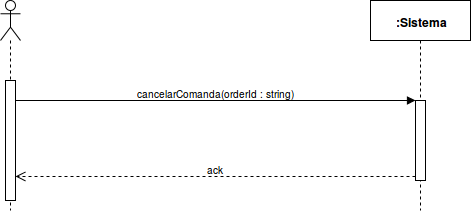
\includegraphics[scale=0.6]{Figures/casdus_11.png}
\caption{Esquema de comportament del cas d'ús \#11}
\end{figure}
\begin{table}[h]
\noindent
\begin{tabularx}{\linewidth}{
>{\hsize=.2\hsize}X% 10% of 4\hsize 
>{\hsize=0.8\hsize}X% 30% of 4\hsize
}
\textbf{Context} 		& Sistema :: cancelarComanda(orderId : string) \\
\textbf{Precondició} 	& La comanda amb id \textit{orderId} existeix dins la base de dades. \\
\textbf{Postcondició}	& L'aplicació cancel·la la comanda eliminant tota instància relacionada amb ella. \\
\end{tabularx}
\label{}
\end{table}

\noindent\textbf{\large Cas d'ús \#12}\\
\begin{figure}[H]
\centering
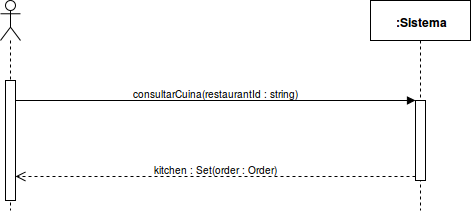
\includegraphics[scale=0.6]{Figures/casdus_12.png}
\caption{Esquema de comportament del cas d'ús \#12}
\end{figure}
\begin{table}[h]
\noindent
\begin{tabularx}{\linewidth}{
>{\hsize=.2\hsize}X% 10% of 4\hsize 
>{\hsize=0.8\hsize}X% 30% of 4\hsize
}
\textbf{Context} 		& Sistema :: consultarCuina(restaurantId : string) \\
\textbf{Precondició} 	& El restaurant amb id \textit{restaurantId} existeix dins la base de dades. \\
\textbf{Postcondició}	& L'aplicació mostra totes les comandes les quals encara existeix algun ítem que no ha estat preparat. \\
\end{tabularx}
\label{}
\end{table}

\clearpage
\noindent\textbf{\large Cas d'ús \#13}\\
\begin{figure}[H]
\centering
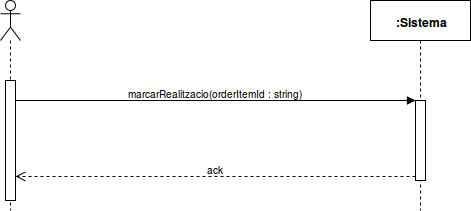
\includegraphics[scale=0.6]{Figures/casdus_13.png}
\caption{Esquema de comportament del cas d'ús \#13}
\end{figure}
\begin{table}[h]
\noindent
\begin{tabularx}{\linewidth}{
>{\hsize=.2\hsize}X% 10% of 4\hsize 
>{\hsize=0.8\hsize}X% 30% of 4\hsize
}
\textbf{Context} 		& Sistema :: marcarRealitzacio(orderItemId : string) \\
\textbf{Precondició} 	& La línia de comanda amb id \textit{orderItemId} existeix dins la base de dades. \\
\textbf{Postcondició}	& L'aplicació marca l'ítem com a realitzat i mostra l'actualització. \\
\end{tabularx}
\label{}
\end{table}

\noindent\textbf{\large Cas d'ús \#14}\\
\begin{figure}[H]
\centering
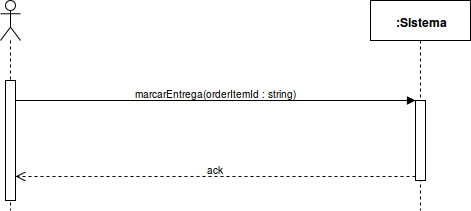
\includegraphics[scale=0.6]{Figures/casdus_14.png}
\caption{Esquema de comportament del cas d'ús \#14}
\end{figure}
\begin{table}[h]
\noindent
\begin{tabularx}{\linewidth}{
>{\hsize=.2\hsize}X% 10% of 4\hsize 
>{\hsize=0.8\hsize}X% 30% of 4\hsize
}
\textbf{Context} 		& Sistema :: marcarEntrega(orderItemId : string) \\
\textbf{Precondició} 	& La línia de comanda amb id \textit{orderItemId} existeix dins la base de dades. \\
\textbf{Postcondició}	& L'aplicació marca l'ítem com a entregat i mostra l'actualització. \\
\end{tabularx}
\label{}
\end{table}

\clearpage
\noindent\textbf{\large Cas d'ús \#15}\\
\begin{figure}[H]
\centering
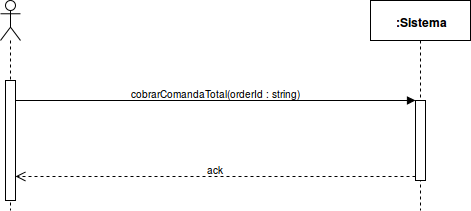
\includegraphics[scale=0.6]{Figures/casdus_15.png}
\caption{Esquema de comportament del cas d'ús \#15}
\end{figure}
\begin{table}[h]
\noindent
\begin{tabularx}{\linewidth}{
>{\hsize=.2\hsize}X% 10% of 4\hsize 
>{\hsize=0.8\hsize}X% 30% of 4\hsize
}
\textbf{Context} 		& Sistema :: cobrarComandaTotal(orderId : string) \\
\textbf{Precondició} 	& La comanda amb id \textit{orderId} existeix dins la base de dades. \\
\textbf{Postcondició}	& L'aplicació indica per tot ítem de la comanda el seu nou estat de cobrat i mostra l'actualització. \\
\end{tabularx}
\label{}
\end{table}

\noindent\textbf{\large Cas d'ús \#16}\\
\begin{figure}[H]
\centering
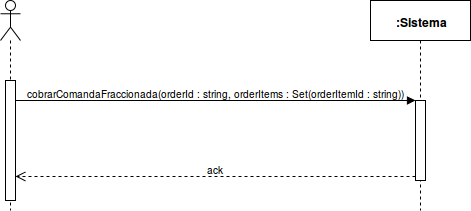
\includegraphics[scale=0.6]{Figures/casdus_16.png}
\caption{Esquema de comportament del cas d'ús \#16}
\end{figure}
\begin{table}[h]
\noindent
\begin{tabularx}{\linewidth}{
>{\hsize=.2\hsize}X% 10% of 4\hsize 
>{\hsize=0.8\hsize}X% 30% of 4\hsize
}
\textbf{Context} 		& Sistema :: cobrarComandaFraccionada(orderId : string,\\
						& orderItems : Set(orderItemId : string)) \\
\textbf{Precondició} 	& La comanda amb id \textit{orderId} i les línies de comanda amb id \textit{orderItemId} existeixen dins la base de dades. \\
\textbf{Postcondició}	& L'aplicació marca com a pagades totes les línies de comanda seleccionades i mostra l'actualització. \\
\end{tabularx}
\label{}
\end{table}

\clearpage
\noindent\textbf{\large Cas d'ús \#17}\\
\begin{figure}[H]
\centering
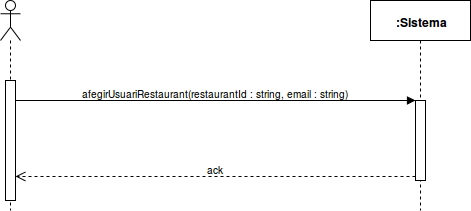
\includegraphics[scale=0.6]{Figures/casdus_17.png}
\caption{Esquema de comportament del cas d'ús \#17}
\end{figure}
\begin{table}[h]
\noindent
\begin{tabularx}{\linewidth}{
>{\hsize=.2\hsize}X% 10% of 4\hsize 
>{\hsize=0.8\hsize}X% 30% of 4\hsize
}
\textbf{Context} 		& Sistema :: afegirUsuariRestaurant(restaurantId : string,\\
						& email : string) \\
\textbf{Precondició} 	& El restaurant amb id \textit{restaurantId} existeix dins la base de dades i el correu electrònic \textit{email} és vàlid. \\
\textbf{Postcondició}	& L'aplicació afegeix l'usuari amb correu electrònic \textit{email} dins el restaurant especificat en cas que no formi part de cap altre restaurant i existeix a la base de dades, altrament ho notifica i no realitza cap canvi. \\
\end{tabularx}
\label{}
\end{table}

\noindent\textbf{\large Cas d'ús \#18}\\
\begin{figure}[H]
\centering
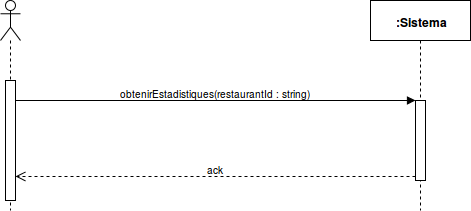
\includegraphics[scale=0.6]{Figures/casdus_18.png}
\caption{Esquema de comportament del cas d'ús \#18}
\end{figure}
\begin{table}[h]
\noindent
\begin{tabularx}{\linewidth}{
>{\hsize=.2\hsize}X% 10% of 4\hsize 
>{\hsize=0.8\hsize}X% 30% of 4\hsize
}
\textbf{Context} 		& Sistema :: obtenirEstadistiques(restaurantId : string) \\
\textbf{Precondició} 	& El restaurant amb id \textit{restaurantId} existeix dins la base de dades. \\
\textbf{Postcondició}	& L'aplicació mostra tota la informació estadística relacionada amb el restaurant. \\
\end{tabularx}
\label{}
\end{table}

\clearpage
\noindent\textbf{\large Cas d'ús \#19}\\
\begin{figure}[H]
\centering
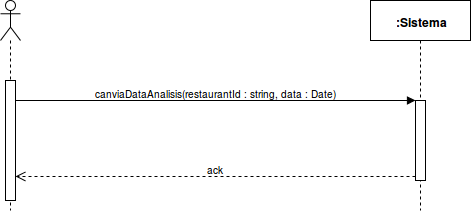
\includegraphics[scale=0.6]{Figures/casdus_19.png}
\caption{Esquema de comportament del cas d'ús \#19}
\end{figure}
\begin{table}[h]
\noindent
\begin{tabularx}{\linewidth}{
>{\hsize=.2\hsize}X% 10% of 4\hsize 
>{\hsize=0.8\hsize}X% 30% of 4\hsize
}
\textbf{Context} 		& Sistema :: canviaDataAnalisis(restaurantId : string,\\
						& data : Date) \\
\textbf{Precondició} 	& El restaurant amb id \textit{restaurantId} existeix dins la base de dades i la data \textit{date} és vàlida. \\
\textbf{Postcondició}	& L'aplicació calcula de nou les estadístiques amb la nova data \textit{date} i mostra l'actualització. \\
\end{tabularx}
\label{}
\end{table}

\noindent\textbf{\large Cas d'ús \#20}\\
\begin{figure}[H]
\centering
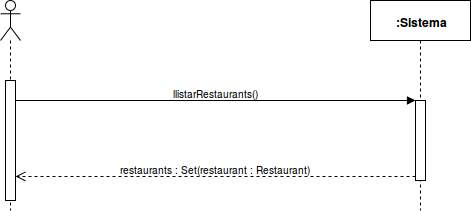
\includegraphics[scale=0.6]{Figures/casdus_20.png}
\caption{Esquema de comportament del cas d'ús \#20}
\end{figure}
\begin{table}[h]
\noindent
\begin{tabularx}{\linewidth}{
>{\hsize=.2\hsize}X% 10% of 4\hsize 
>{\hsize=0.8\hsize}X% 30% of 4\hsize
}
\textbf{Context} 		& Sistema :: llistarRestaurants() \\
\textbf{Precondició} 	& - \\
\textbf{Postcondició}	& L'aplicació mostra un llistat amb tots els restaurant emmagatzemats dins l'aplicació. \\
\end{tabularx}
\label{}
\end{table}

\clearpage
\noindent\textbf{\large Cas d'ús \#21}\\
\begin{figure}[H]
\centering
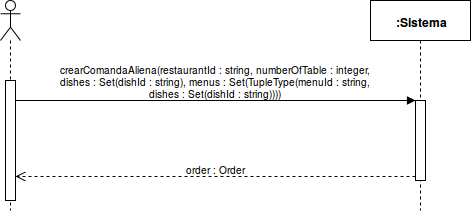
\includegraphics[scale=0.6]{Figures/casdus_21.png}
\caption{Esquema de comportament del cas d'ús \#21}
\end{figure}
\begin{table}[h]
\noindent
\begin{tabularx}{\linewidth}{
>{\hsize=.2\hsize}X% 10% of 4\hsize 
>{\hsize=0.8\hsize}X% 30% of 4\hsize
}
\textbf{Context} 		& Sistema :: crearComandaAliena(restaurantId : string, \\
						& numberOfTable : integer, \\
						& dishes : Set(dishId : string), \\
						& menus : Set(TupleType(menuId : string, \\
						& dishes : Set(dishId : string)))) \\
\textbf{Precondició} 	& El restaurant amb id \textit{restaurantId}, els plats amb id \textit{dishId} i els menus amb id \textit{menuId} existeixen dins la base de dades. \\
\textbf{Postcondició}	& L'aplicació emmagatzema la informació indicada als paràmetres, indica la comanda com a externa dins al restaurant i mostra la comanda creada. \\
\end{tabularx}
\label{}
\end{table}

\noindent\textbf{\large Cas d'ús \#22}\\
\begin{figure}[H]
\centering
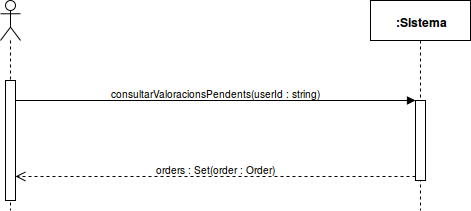
\includegraphics[scale=0.6]{Figures/casdus_22.png}
\caption{Esquema de comportament del cas d'ús \#22}
\end{figure}
\begin{table}[h]
\noindent
\begin{tabularx}{\linewidth}{
>{\hsize=.2\hsize}X% 10% of 4\hsize 
>{\hsize=0.8\hsize}X% 30% of 4\hsize
}
\textbf{Context} 		& Sistema :: consultarValoracionsPendents(userId : string) \\
\textbf{Precondició} 	& L'usuari amb id \textit{userId} existeix dins la base de dades. \\
\textbf{Postcondició}	& L'aplicació mostra el conjunt de comandes que estan pendents de valorar. \\
\end{tabularx}
\label{}
\end{table}

\clearpage
\noindent\textbf{\large Cas d'ús \#23}\\
\begin{figure}[H]
\centering
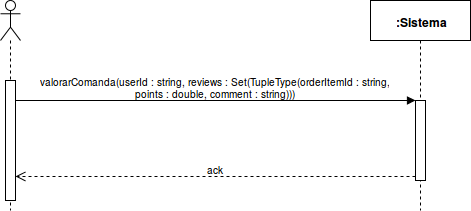
\includegraphics[scale=0.6]{Figures/casdus_23.png}
\caption{Esquema de comportament del cas d'ús \#23}
\end{figure}
\begin{table}[h]
\noindent
\begin{tabularx}{\linewidth}{
>{\hsize=.2\hsize}X% 10% of 4\hsize 
>{\hsize=0.8\hsize}X% 30% of 4\hsize
}
\textbf{Context} 		& Sistema :: valorarComanda(userId : string\\
						& reviews : Set(TupleType(orderItemId : string, \\
						& points : double, comment : string))) \\
\textbf{Precondició} 	& L'usuari amb id \textit{userId} existeix dins la base de dades. \\
\textbf{Postcondició}	& L'aplicació emmagatzema la valoració i ho notifica a l'usuari. \\
\end{tabularx}
\label{}
\end{table}

\noindent\textbf{\large Cas d'ús \#24}\\
\begin{figure}[H]
\centering
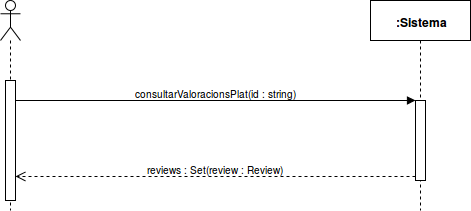
\includegraphics[scale=0.6]{Figures/casdus_24.png}
\caption{Esquema de comportament del cas d'ús \#24}
\end{figure}
\begin{table}[h]
\noindent
\begin{tabularx}{\linewidth}{
>{\hsize=.2\hsize}X% 10% of 4\hsize 
>{\hsize=0.8\hsize}X% 30% of 4\hsize
}
\textbf{Context} 		& Sistema :: consultarValoracionsPlat(id : string) \\
\textbf{Precondició} 	& El plat o el menú amb l'identificador \textit{id} existeix dins la base de dades. \\
\textbf{Postcondició}	& L'aplicació mostra les valoracions de l'element especificat. \\
\end{tabularx}
\label{}
\end{table}

\clearpage
\noindent\textbf{\large Cas d'ús \#25}\\
\begin{figure}[H]
\centering
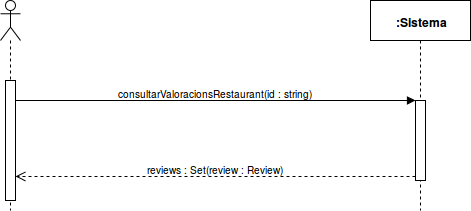
\includegraphics[scale=0.6]{Figures/casdus_25.png}
\caption{Esquema de comportament del cas d'ús \#25}
\end{figure}
\begin{table}[h]
\noindent
\begin{tabularx}{\linewidth}{
>{\hsize=.2\hsize}X% 10% of 4\hsize 
>{\hsize=0.8\hsize}X% 30% of 4\hsize
}
\textbf{Context} 		& Sistema :: consultarValoracionsRestaurant(id : string) \\
\textbf{Precondició} 	& El restaurant amb id \textit{restaurantId} existeix dins la base de dades. \\
\textbf{Postcondició}	& L'aplicació mostra les valoracions del restaurant especificat. \\
\end{tabularx}
\label{}
\end{table}